\documentclass[12pt,pdf,hyperref={unicode}]{beamer}
%\usetheme{boxes}
\beamertemplatenavigationsymbolsempty
\setbeamertemplate{footline}[page number]
% Set it for the internal PhD thesis defence to reduce number of slides
%\setbeamersize{text margin left=0.5em, text margin right=0.5em}

\usepackage[T1]{fontenc}

\usepackage[utf8]{inputenc}
\usepackage[english, russian]{babel}
\usepackage{bm}
\usepackage{multirow}
\usepackage{ragged2e}
\usepackage{indentfirst}
\usepackage{multicol}
\usepackage{subfig}
\usepackage{amsmath,amssymb}
\usepackage{enumerate}
\usepackage{mathtools}
\usepackage{comment}
\usepackage{physics}
\usepackage[all]{xy}
\usepackage{tikz}
\usetikzlibrary{positioning,arrows}
\tikzstyle{name} = [parameters]
\definecolor{name}{rgb}{0.5,0.5,0.5}

% colors
\definecolor{darkgreen}{rgb}{0.0, 0.2, 0.13}
\definecolor{darkcyan}{rgb}{0.0, 0.55, 0.55}
%\AtBeginEnvironment{figure}{\setcounter{subfigure}{0}}
%\captionsetup[subfloat]{labelformat=empty}

%----------------------------------------------------------------------------------------------------------

\title{ Put the title of your thesis \\ here}
%\author{Name Surname}
%\institute[]{}
%\date{2024}

%---------------------------------------------------------------------------------------------------------
\begin{document}
%\begin{frame}
%\titlepage
%\end{frame}
\setcounter{page}{4}%remove here for the title
%----------------------------------------------------------------------------------------------------------
%\section{Please do not use sectioning in the presentations}
\begin{frame}{Вычислительный эксперимент}
\begin{block}{Цель}
Улучшить качество оценки степени тяжести акне и распознавания пораженных участков, провести сравнение метода с предыдущим подходом.
\end{block}
\begin{block}{Данные}
Используются 2 набора данных, размеченных профессиональными дерматологами по определенным критериям.
\begin{itemize}
    \item Датасет ACNE04 из 1457 изображений лиц, для каждого известна оценка $S \in [0, 1]$ степени тяжести акне и набор bounding boxes для пораженных участков.
    \item Набор из 668 фотопортретов с соответсвующими оценками степени тяжести акне $S \in [0, 1]$.
\end{itemize}
\end{block}
\end{frame}
%----------------------------------------------------------------------------------------------------------
\begin{frame}{Зависимость качества от параметров и моделей}
\begin{columns}
\begin{column}{0.5\textwidth}
    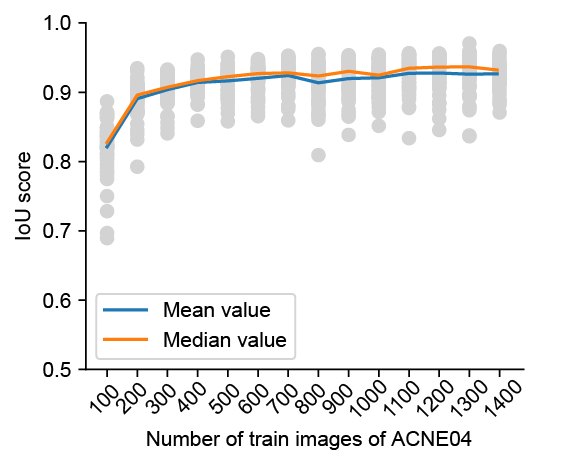
\includegraphics[width=1\textwidth]{Holicheva-Step-10-fig-1}
\end{column}
\begin{column}{0.5\textwidth}
	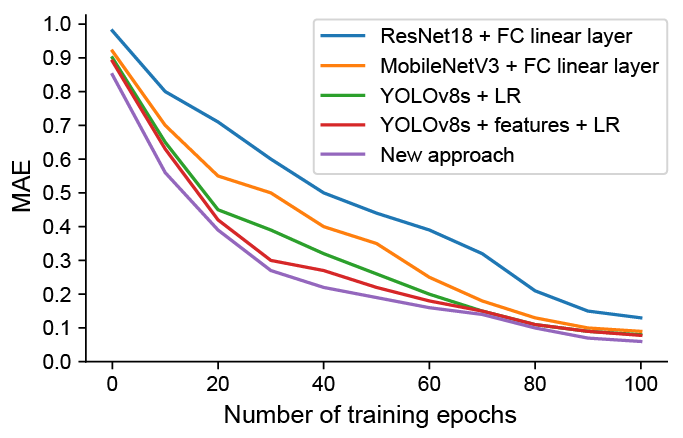
\includegraphics[width=1\textwidth]{Holicheva-Step-10-fig-2}      
\end{column}
\end{columns}
\begin{itemize}
    \item Исследование зависимости качества от размера обучающей выборки позволяет установить ее оптимальный размер.
    \item Создание дополнительных признаков в комбинации с современными архитектурами обеспечивает высокое качество решения задачи.
\end{itemize}
\end{frame}
\end{document}